\chapter{Word Embedding}
Word embeddings is distributed representation of words in a vector space. With the learning algorithm it can capture the contextual or co-occurrence information. The word embedding has an interesting and important property: similar words will have similar distribution in the embedding space, with that property, we can find meaningful near-synonyms or  Some successful methods for learning word embedding like word2vec\cite{mikolov2013distributed}, \cite{pennington2014glove}

\section{Monolingual Embedding}
\begin{figure}[h]
	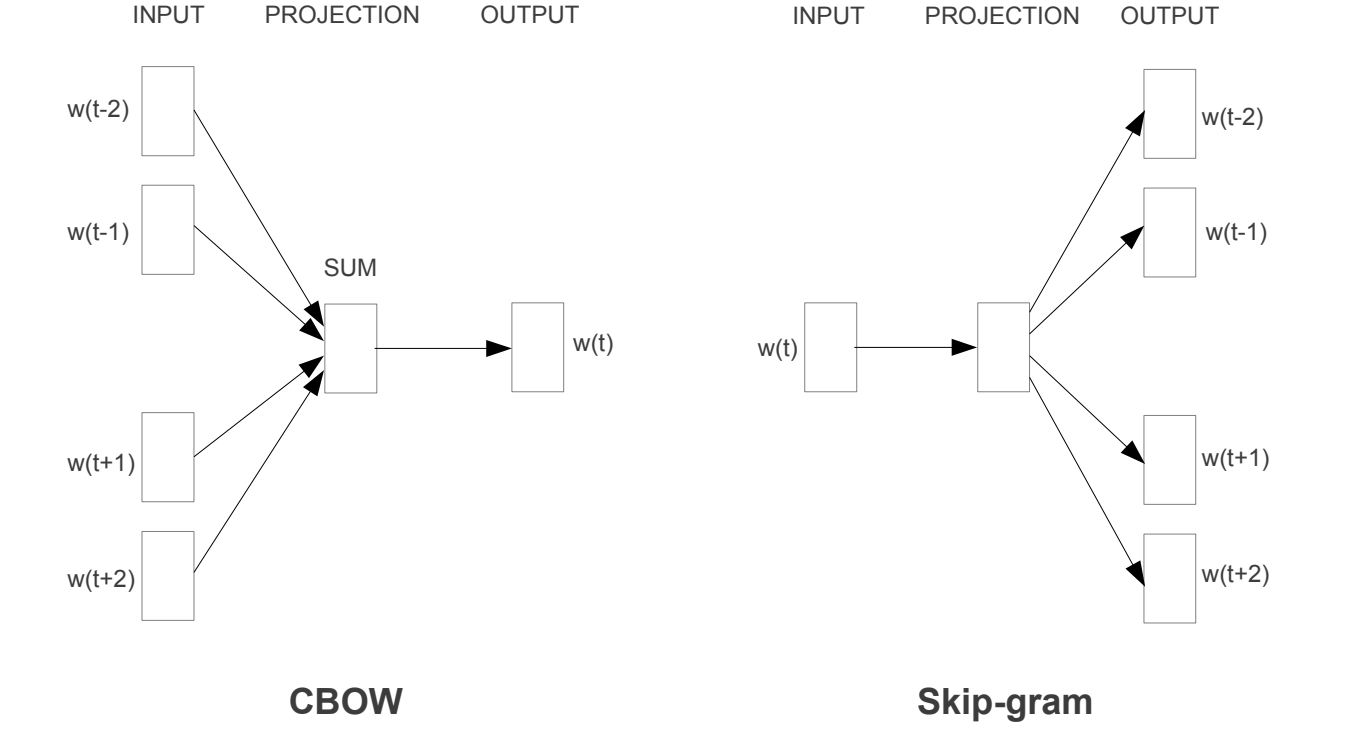
\includegraphics[width=12cm]{word2vec}
	\caption{Global attention model (\cite{mikolov2013efficient})}
	\centering
\end{figure}
\subsection{CBOW and Skip-gram Model}
CBOW model and skip-gram model are currently mainstream neural network to learn the word embedding. Algorithmically,  CBOW tries to predict the current word based on the context while skip-gram model is to find better representations that are useful for predicting the surrounding words. Using skip-gram model as example, given a large training corpus represented as a sequence of words ${e_1, \cdots e_N}$, the objective of the model is to maximize the following log-likelihood:
\[ \frac{1}{I} \sum_{i=1}^{I} \sum_{ -c \le j \le c, j\ne 0} \log\ {p(e_{i+j}|e_i)} \]
where $e_i$ is the current word and $c$ is the size of training context. \\
We define the loss for skip-gram model as
\[ \mathcal{L}^e_{\text{skip-gram}} = - \frac{1}{I} \sum_{i=1}^{I} \sum_{ -c \le j \le c, j\ne 0} \log\ {p(e_{i+j}|e_i)}\]

Similarly, we define the loss for CBOW model as
\[ \mathcal{L}^e_{\text{CBOW}} = - \frac{1}{I} \sum_{i=1}^{I} \sum_{ -c \le j \le c, j\ne 0} \log\ {p(e_{i}|e_{i+j})}\]
Furthermore in skip-gram model, suppose given a scoring function s which maps word pairs to score in $\mathbb{R}0$ like cosine similarity, the probability can be defined as
\[ p(e_{i+j} | e_i)  = \frac{\exp\{s(e_{i+j}, e_j)\}}{\sum_{e^{\prime} \in V^e }{\exp\{s( e^{\prime}, e_i)\}}}\]
where $V^e$ is the whole vocabulary. \\

\textbf{Negative Sampling}\\
However the normalization on the whole vocabulary is very expensive since it is conducted for all words at every training step. Negative sampling is proposed to approximate the softmax to make it computationally more efficient. The problem of predicting words can be considered as an independent binary classification task. Negative sampling trains the model to distinguish a target word from negative samples drawn from a noise  distribution $P_{\text{noise}}$.   
\[p(e_{i+j}|e_i) = \log {Q_{\theta}{(D=1 | e_{i+j}, e_i)}} + \frac{1}{k}\sum_{e^{\prime} \sim P_{\text{noise}}} {\log{Q_{\theta}{(D=0 | e^{\prime}, e_i )}}}  \]

where ${Q_{\theta}{(D=1| w_t, w_s)}}$ is the binary logistic regression probability.
According to  empirical results, CBOW works better on smaller datasets because CBOW smoothes over a lot of the distributional information while Skip-Gram model performs better when we have larger datasets

\subsection{FastText}
The training methods above treat each word as a distinct word embedding, however intuitively we can obtain more information from the morphological information of words. A subword model was proposed to try to fix such problem.The training network is similar, the model design a new presentation of the word: it adds speicial symbols $<$, ${>}$ as boundary information at the beginning and the end of a word. Then a normal word is represented as a bag of character $n$-grams . For example the word "where" and n equals 3, the it can be represented as the following 5 tri-grams: 
\[ <wh, whe, her, ere, re>\]
Suppose in this way for a specific word $e$ ${G_{e}}$ the set of character ${n}$-grams, we assign for each character ${n}$-gram $g$ in ${G_{e}}$ a distinct vector $\bm{v}_g$, we calculate the score function using the sum of character-level inner product of vectors:
\[s(e^{\prime}, e) = \sum_{g \in G_{e}} \bm{v}_g^{T} \bm{e}^{\prime} \]
where $\bm{e}^{\prime}$ the embedding of $e^{\prime}$
\section{ Cross-lingual Word Embedding}
 NLP tasks in multilingual scenarios is receiving increasing interest. The need to represent meaning and transfer knowledge in cross-lingual applications has motivated the works on cross-lingual models which learns the representations in a joint embedding space. Mikolov  observe that word embeddings trained separately on monolingual corpora exhibits isomorphic structure across languages, as illustrated in Figure $3.2$. That means we can create a connection between source embedding and target embedding even with simple linear mapping. This has far-reaching implication on low-resource scenarios (\cite{adams2017cross}), because word embedding requires only plain text to train, which is the most abundant form of linguistic resource.
\begin{figure}[t]
	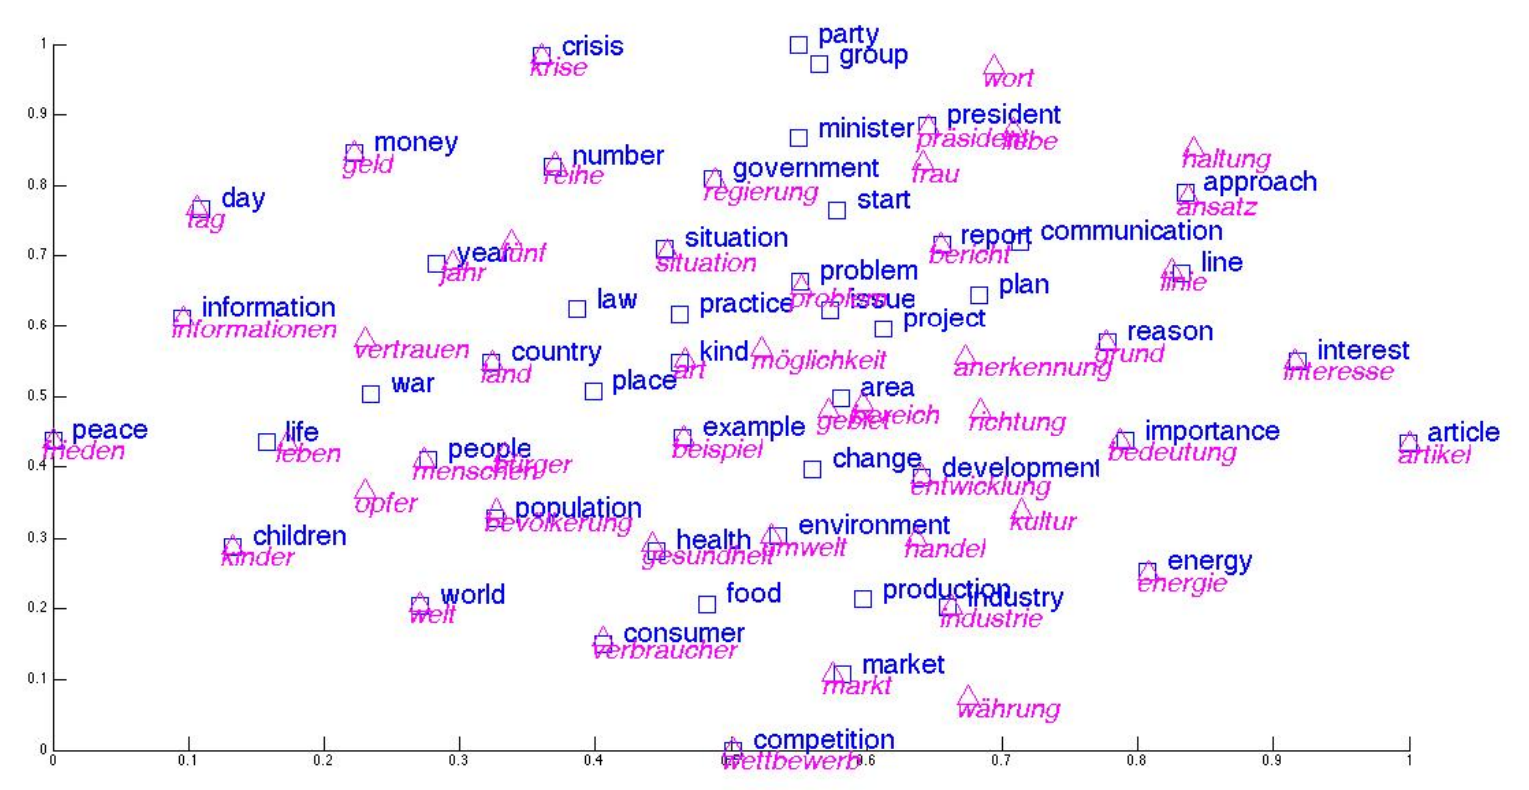
\includegraphics[width=14cm]{crossembedding}
	\centering
	\caption{A cross-lingual embedding space between German and English (\cite{ruder2017survey})}
\end{figure}

%In the thesis, I assume there are two set of embeddings ${e}$, ${f}$trained separately on monolingual data.  The propose of cross-lingual word embedding training is to learn such a mapping ${W \in }$ from source embedding space to target embedding space, so $Wf_i, e_j$ in the same embedding space and for all corresponding word pairs, we need to optimize the mapping ${W}$, so that"
%
%
%\[ \arg\min_{W \in R^{d \times d}} \sum_{i} \lVert Wf_i - e_i \rVert \]
%where $d$ is the dimension of embeddings, and the distance ${\lVert Wf_i - e_i \rVert}$ can be different types. We prefer the Euclidean distance.  
%
%first
	

\subsection{Training Algorithm}
Most training methods can be divided into joint training approaches and mapping-based approaches. The difference is that joint methods train directly the cross-lingual word embedding while the mapping-based approaches first train monolingual word representations on corresponding corpus separately. Then mappings are learned to project different embeddings into the shared space. They learn the transformation from word alignments or bilingual dictionaries. \\

\textbf{Joint Training Approaches}\\
Joint training means to optimize the source and target embeddings objectives $\mathcal{L(\cdot)}$ jointly with the cross-lingual regularization term $\Omega(\cdot)$. 
\[ \mathcal{L} =  \mathcal{L}_{\text{skip-gram}}^e + \mathcal{L}_{\text{skip-gram}}^f + \lambda \cdot \Omega(\cdot)  \]
where the first two losses are exact the same as those in monolingual embedding training. While the $\Omega(\cdot)$  encourages the similar words representations to be similar for words that are related across different languages.

Different cross-lingual regularization terms are proposed to optimize the cross-lingual embeddings (\cite{coulmance2016trans}, \cite{luong2015bilingual}, \cite{gouws2015bilbowa}). For example, \cite{gouws2015bilbowa} models it as: 
\[ \Omega_{\text{BilBOWA}} = {\lVert \frac{1}{I}  \sum_{e_i \in e_1^I} \bm{e}_i - \frac{1}{J} \sum_{f_j \in f_1^J} \bm{f}_j\rVert}^2 \]
where $\bm{f}_j$ and $\bm{e}_i$ are the word embeddings for words in parallel source and target sentences. Instead of relying on expensive word alignments which minimize the distance that aligned to each other, they minimize the distance between the mean of the word representations in the aligned sentences. \\

\textbf{Mapping-based Approaches}: \\
There are two methods to learn the cross-lingual word embedding, one is to learn the transformation for each language, both monolingual embeddings are mapped into a shared embedding space. The typical model is CCA-based approaches (\cite{faruqui2014improving}, \cite{dhillon2011multi} and \cite{lu2015deep}). The other method is to learn the mapping from the source embedding space to the target embedding space. The criterion is to minimize the mean squared error between the transformed source embeddings and the target embeddings. The advantage of this method is that it is really fast to learn the embedding alignments. People criticize whether linear or nonlinear can capture the relationship between all words in different languages.


\subsubsection{Canonical Correlation Analysis (CCA)}
\begin{figure}[t]
	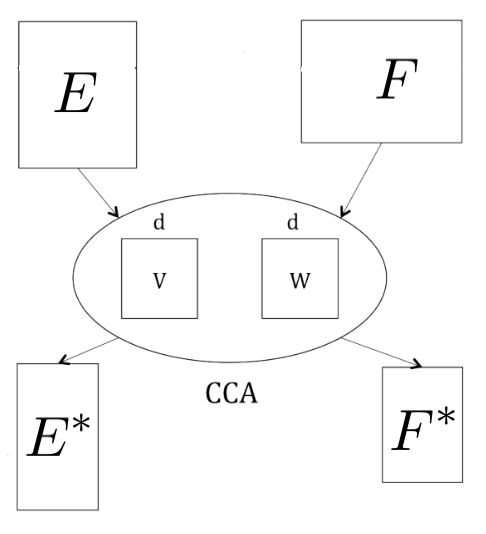
\includegraphics[width=8cm]{cca}
	\centering
	\caption{Cross-lingual projection with CCA (\cite{faruqui2014improving})}
\end{figure}
let $F^{\prime} \in \mathbb{R}^{d_1 \times n}$ and $E^{\prime} \in \mathbb{R}^{d_2 \times n}$ be the embedding matrices comprised of seed word translation pairs with size $n$. The  $W$ and $V$ are the projection matrices which mapped the original embedding matrices into $F^{*}$ and $E^{*}$, which are in the joint space.

\[ {F}^{*} = W {F^{\prime}} \ \ \ \  {E}^{*} = V{E^{\prime}} \] 
The objective of CCA is to find the two matrices such that the projections of the parallel matrices are maximally correlated:
\[ \argmax{W \in \mathbb{R}, V in \mathbb{R}} \frac{\mathbb{E}[({F}^{*})({E}^{*})]}{\sqrt{\mathbb{E}[({F}^{*})^2]} \sqrt{\mathbb{E}[({E}^{*})^2]}} \]
Once we get the two projection matrices, we can calculate the cross-lingual word embedding for the entire vocabulary.

A linear feature mapping is often not sufficiently powerful to faithfully capture the hidden, non-linear relations within the data. \cite{lu2015deep} propose a non-linear extension of CCA using deep neural networks, where two neural networks are used to extract features separately, and trained to maximize the correlations between these features, measured by a linear CCA step with projection mappings the neural network weights and linear projections are optimized together. Different from CCA, the neural network model does not have a closed-form solution, the parameters can be learned via gradient-based optimization.
\[ \]
%where $W_f$ and $W_e$ are the weights of the two networks and ${}$ ${}$, ${}$ are covariance matrices computed for   in the ssame way as CCA. The final transformation is the composition of the neural network ans CCA projection, $\bm{u}^T \bm{f}$ for the view. The algorithm does not have a closed-form solution but the parameters can be learned via gradient-based optimization with mini-batch stochastic gradient descent .
%\begin{enumerate}
%	\item Mapping based approaches\\
%	First train the monolingual word embedding separately and then seek the seed dictionary to learn the mapping. 
%	\item Pseudo-multi-lingual corpora-based approaches\\
%	Use the monolingual embedding training method on constructed corpora that contains both the source and the target language.
%	\item Joint methods\\
%	Take the parallel text as input and minimize the source and target language losses jointly with the cross-lingual regularization term
%\end{enumerate}


\subsubsection{Cross-lingual Mapping}
\cite{mikolov2013exploiting} notice that the geometric relation that hold between words are similar across languages. This suggest that, we can jump the third embedding space, learn the transformation directly from source embedding space to target space.
Given a seed word translation pair set $d$ of size $n$, the objective is to learn $W$ that minimizes the distance between the mapped source word embedding $W\bm{f}_i$ and target embedding $\bm{e}_i$:
\[ \argmin{W} \sum_{\substack{i=1\\ (\bm{f}_i, \bm{e}_i) \in d} }^n {\lVert W\bm{f}_i - \bm{e}_i \rVert}_2^2 \]
This can also be expressed in matrix form as minimizing the squared Frobenius norm of the residual matrix:
\[ \argmin{W} {\ \lVert WF - E \rVert}_F^2 \]



 \cite{xing2015normalized} showed that the results are improved when we use $l_2$ normalized embeddings and constrain the ${W}$ to be an orthogonal matrix. In this case we can use Procrustes analysis which advantageously offers a closed form solution obtained from the singular value decomposition 
\[W^* = \argmin{W \in O_d(\mathbb{R})} {\ \lVert WF - E \rVert}_F^2 = UV^T , \quad U\Sigma V^T = SVD(EF^T) \]

In order to make learning and inference consistent, \cite{DBLP:journals/corr/abs-1804-07745} propose the relaxed CSLS loss (RCSLS), which is inspired from the work of \cite{conneau2017word}

The loss function can be rewritten as:
\[ \min_{\bm{W} \in \mathcal{O}_d} = \frac{1}{n} \sum_{i=1}^{n} \Big\{ -2 \bm{f}_i^\top W^\top \bm{e}_i + \frac{1}{k} \sum_{\bm{e}_j \in \mathcal{N}_e(W\bm{f}_i)} \bm{f}_i^\top W^\top \bm{e}^j + \frac{1}{k} \sum_{W\bm{f}_j \in \mathcal{N}_f(\bm{e}_i)} \bm{f}_j^\top W^\top \bm{e}^i  \Big\}\]


Normally, the size $n$ of the dictionary is too small with respect to the entire vocabulary size, in order to incorporate unlabeled data, the unpaired words in the dictionary are used as "negatives samples" in the RCSLS loss, as result, we can optimize the loss function not only the dictionary but the whole vocabulary.

	
	